\documentclass[tikz,border=2pt]{standalone}
\usepackage{amsmath,amssymb}
\usepackage{pgfplots}
\pgfplotsset{compat=1.18}

\begin{document}
% Chebyshev bounds the two tails |X - mu| >= a together by sigma^2/a^2, whatever the shape of
% the distribution; for a = 2 sigma the bound is 1/4 (the true normal tail mass is 0.046).
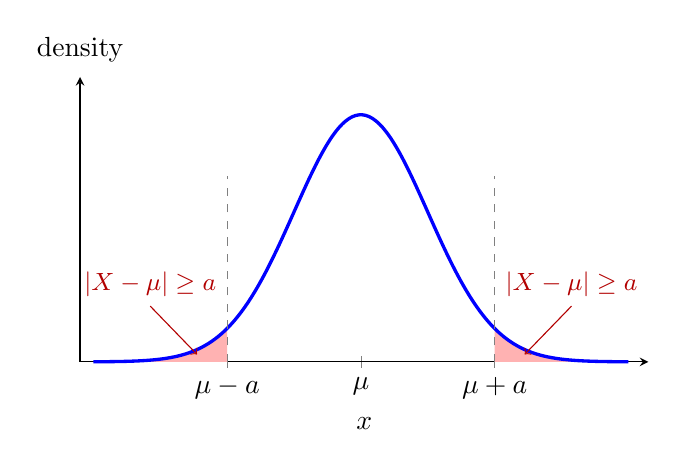
\begin{tikzpicture}
	\begin{axis}[
		axis lines=left, xmin=-4.2, xmax=4.3, ymin=0, ymax=0.46,
		xtick={-2,0,2}, xticklabels={$\mu-a$,$\mu$,$\mu+a$}, ytick=\empty,
		xlabel={$x$}, ylabel={density}, ylabel style={rotate=-90, anchor=south, at={(axis description cs:0,1.02)}},
		samples=160, smooth, width=8.8cm, height=5.2cm, clip=false
		]
		\addplot[fill=red!30, draw=none, domain=-4:-2] {exp(-x^2/2)/sqrt(2*pi)} \closedcycle;
		\addplot[fill=red!30, draw=none, domain=2:4] {exp(-x^2/2)/sqrt(2*pi)} \closedcycle;
		\addplot[blue, very thick, domain=-4:4] {exp(-x^2/2)/sqrt(2*pi)};
		\draw[gray, dashed] (axis cs:-2,0) -- (axis cs:-2,0.3);
		\draw[gray, dashed] (axis cs:2,0) -- (axis cs:2,0.3);
		\node[red!70!black, font=\small, anchor=south] at (axis cs:-3.15,0.09) {$|X-\mu|\ge a$};
		\node[red!70!black, font=\small, anchor=south] at (axis cs:3.15,0.09) {$|X-\mu|\ge a$};
		\draw[red!70!black, ->] (axis cs:-3.15,0.09) -- (axis cs:-2.45,0.012);
		\draw[red!70!black, ->] (axis cs:3.15,0.09) -- (axis cs:2.45,0.012);
	\end{axis}
	
\end{tikzpicture}
\end{document}
